\documentclass[twocolumn]{article}
\usepackage{graphicx}
\usepackage{url}
\usepackage{amsmath}
\usepackage{amssymb}
\usepackage{amsfonts}
\usepackage{color}
\usepackage[utf8]{inputenc}
\usepackage[T1]{fontenc}
\usepackage{float}
\usepackage{subcaption}
\usepackage{caption}
\usepackage{booktabs}
\usepackage{geometry}
\usepackage{multirow}
\usepackage{hyperref}
\geometry{margin=2.5cm}
\usepackage{authblk}
\usepackage{tikz}
\usetikzlibrary{shapes.geometric,arrows.meta,positioning,fit,backgrounds,calc}

%%
\title{Hierarchical Coarse-to-Fine RAG for Japanese Civil-Engineering Standards:\\
A Comparative Study of Naive, Hybrid, and Structure-Aware Retrieval\\
on River and Sediment Control Technical Documents}

\author[1]{Takato Yasuno}
%\affil[1]{Affiliation}
%\affil[ ]{Email: }

\date{}

\begin{document}
\maketitle

%% ====================================================================
\begin{abstract}
%% ====================================================================

Answering precise technical questions against Japan's multi-volume
\textbf{River and Sediment Control Technical Standards} requires retrieving
highly specific passages from a document corpus with rich hierarchical structure
(volumes, chapters, and sections) under the strict constraint of a single
consumer-grade GPU (16~GB VRAM).
This paper presents a systematic comparison of three retrieval-augmented generation (RAG)
strategies applied to this domain:

\noindent\textbf{Naive RAG} (flat dense vector search, FAISS IndexFlatIP),
\textbf{Light RAG} (hybrid BM25 + dense fusion with $\alpha = 0.5$), and
\textbf{HippoRAG2-Hier} (a knowledge-graph-free hierarchical coarse-to-fine strategy
that exploits the Volume $\to$ Chapter $\to$ Chunk structure of the standards through
cascaded representative-vector selection).

Each retrieval strategy is paired with two open-source Japanese LLMs
served locally via Ollama---Swallow-8B-LoRA-Q4 and ELYZA-JP-8B-LoRA-Q4---yielding
\textbf{six conditions} evaluated on a \textbf{200-question benchmark} (seed=42).
Answers are scored automatically by Qwen2.5-7B-Instruct as AI-as-Judge
on a 0--3 rubric measuring technical accuracy and standard citation quality.

Our results demonstrate that HippoRAG2-Hier consistently outperforms both baselines
in judge average score and perfect-score rate while remaining within the 16~GB VRAM
budget. The hierarchical pre-filtering reduces irrelevant chunk retrieval
and concentrates context on technically relevant sections.
Light RAG provides a stronger keyword-recall advantage than Naive RAG on
definition-style questions but underperforms on procedure-centric questions
where document structure matters more than term frequency.
We also find that LLM choice interacts with retrieval strategy:
ELYZA-JP-8B-LoRA gains more from structural retrieval augmentation than
Swallow-8B-LoRA, whose domain LoRA training partially compensates for
weaker retrieval.

\end{abstract}

\noindent
\textbf{Keywords:} Retrieval-Augmented Generation, Hierarchical RAG,
BM25 Hybrid Retrieval, Japanese NLP, River Engineering, Technical Standards,
LLM-as-Judge, Open-Source LLM, Domain Adaptation, Civil Engineering AI.

%% ====================================================================
\section{Introduction}
\label{sec:intro}
%% ====================================================================

Japan's \emph{River and Sediment Control Technical Standards}
(\textit{Kasen Sabo Gijutsu Kijun}), issued by the Ministry of Land, Infrastructure,
Transport and Tourism (MLIT), span eight volumes covering survey methodology,
planning procedures, structural design criteria, and maintenance protocols for
river levees, dams, sabo (torrent-control) structures, and related facilities.
Practitioners---field engineers, inspection officers, and dam operators---routinely
require rapid, authoritative answers to highly specific questions embedded in
these multi-hundred-page standards:
inspection intervals, load calculation assumptions, maintenance-planning hierarchies,
and hazard-response decision trees.

\paragraph{The retrieval challenge.}
Modern large language models (LLMs) trained on general corpora cannot reliably recall
domain-specific regulatory values, section-level procedural constraints, or the
precise hierarchy of Japanese civil-engineering standards.
Retrieval-Augmented Generation (RAG)~\cite{lewis2020rag} addresses this by supplying
retrieved passage context at inference time.
However, \emph{flat} dense vector retrieval---querying all chunks simultaneously---
dilutes retrieval precision in hierarchically structured corpora: the top-$k$ results
may span multiple unrelated volumes, causing the LLM to generate hedged or
off-topic responses.

\paragraph{Hierarchical structure as a retrieval prior.}
The River and Sediment Control Technical Standards are organised in a natural
three-level hierarchy:
\emph{Volume} (eight distinct technical areas)
$\to$ \emph{Chapter} (100+ chapters across all volumes)
$\to$ \emph{Chunk} (paragraph-level text segments of $\approx$500 characters).
This structure provides a powerful coarse-to-fine retrieval prior:
a question about sabo-dam design maintenance is unlikely to require context from
the river-levee survey volume.
HippoRAG~\cite{gutiontov2024hipporag2} proposes graph-based hippocampal memory
structures for LLM retrieval; our work adapts this spirit to a knowledge-graph-free
hierarchical strategy that remains deployable under strict VRAM constraints.

\paragraph{Research questions.}
This paper addresses three questions:
\begin{enumerate}
  \item Does hierarchical coarse-to-fine retrieval outperform flat dense retrieval
        on a highly structured Japanese regulatory corpus?
  \item Does BM25-dense hybrid (Light RAG) provide complementary benefits to
        dense-only Naive RAG in this domain?
  \item How do LLM choice and retrieval strategy interact in determining
        answer quality?
\end{enumerate}

\paragraph{Contributions.}
\begin{enumerate}
  \item A reproducible six-condition benchmark comparing Naive RAG, Light RAG,
        and HippoRAG2-Hier on 200 questions from the River and Sediment Control
        Technical Standards, evaluated by AI-as-Judge scoring.
  \item HippoRAG2-Hier: a knowledge-graph-free hierarchical RAG design that
        exploits document-structure metadata (Volume $\to$ Chapter $\to$ Chunk)
        via cascaded representative-vector selection, fitting within a 16~GB
        VRAM constraint.
  \item An empirical analysis of the interaction between retrieval strategy and
        LLM model choice (Swallow-8B-LoRA vs.\ ELYZA-JP-8B-LoRA) in Japanese
        technical QA.
  \item Open-source implementation of all retrieval strategies and evaluation
        pipelines, with reproducible scripts for index construction, evaluation,
        and visualisation.
\end{enumerate}

Figure~\ref{fig:overview} provides a bird's-eye view of the complete
seven-stage pipeline, from source documents through index construction,
the six-condition evaluation matrix, LLM generation, AI-as-Judge scoring,
to final aggregation.

Section~\ref{sec:related} reviews related work.
Section~\ref{sec:problem} defines the task formally.
Section~\ref{sec:corpus} describes the document corpus and chunking strategy.
Section~\ref{sec:method} details the three retrieval strategies.
Section~\ref{sec:experiments} presents the experimental setup.
Section~\ref{sec:results} reports quantitative results.
Section~\ref{sec:analysis} provides qualitative analysis.
Section~\ref{sec:discussion} discusses implications and limitations.
Section~\ref{sec:conclusion} concludes.

%% ====================================================================
\section{Related Work}
\label{sec:related}
%% ====================================================================

\subsection{Retrieval-Augmented Generation}

Lewis et al.~\cite{lewis2020rag} introduce RAG, combining dense passage retrieval
with sequence-to-sequence generation, demonstrating strong performance on
open-domain knowledge-intensive NLP tasks.
Gao et al.~\cite{gao2024ragsurvey} survey the RAG landscape, categorising
retrieval granularity (chunk, sentence, entity), augmentation strategies,
and generation paradigms across diverse domains.
HyDE~\cite{gao2023hyde} improves dense retrieval by generating a hypothetical
document from the query and retrieving against it, improving recall on
technical questions where the query vocabulary differs from the passage vocabulary.
Self-RAG~\cite{asai2024selfrag} trains a single model to adaptively retrieve
and self-critique through reflection tokens, outperforming standard RAG across
diverse tasks.

\subsection{Hybrid and Structured Retrieval}

Keyword-dense hybrid retrieval has demonstrated consistent improvements over
pure dense retrieval in low-resource and domain-specific settings.
BM25~\cite{robertson2009bm25} remains a strong sparse-retrieval baseline,
particularly for technical corpora where exact term matches carry high precision.
Formal Hybrid Search benchmarks~\cite{ma2021replication} show that
reciprocal rank fusion (RRF) and linear score interpolation both improve over
either alone, motivating our Light RAG fusion design.
HippoRAG~\cite{gutiontov2024hipporag2} proposes neurobiologically-inspired
long-term memory for LLMs through a graph-based retrieval architecture combining
entity extraction, graph-of-passages linking, and PPR-based context selection.
Our HippoRAG2-Hier draws on the coarse-to-fine spirit of this work but replaces
the knowledge-graph component with hierarchical document-structure metadata,
making it applicable without graph-construction overhead and fitting within
the 16~GB VRAM budget.

\subsection{Domain-Specific RAG for Technical Documents}

Siriwardhana et al.~\cite{siriwardhana2023domainrag} show that domain-adaptive
fine-tuning of the retriever and generator significantly improves RAG performance
on specialised corpora.
RAPTOR~\cite{sarthi2024raptor} builds recursive tree-structured summaries of
documents, enabling coarse-to-fine retrieval through hierarchical summarisation
nodes --- a conceptually related approach that requires additional LLM inference
at index time.
Our approach avoids summarisation overhead by using representative vectors
computed directly from chunk embeddings, enabling index construction in a
single embedding pass.

\subsection{Japanese LLMs and Evaluation}

The Swallow family~\cite{okazaki2024swallow} adapts the Llama~3 architecture to
Japanese through continued pre-training on a large Japanese web corpus.
ELYZA-JP-8B~\cite{elyza2024} is an instruction-tuned Japanese LLM released under
a permissive licence, widely used in Japanese industry RAG applications.
LLM-as-Judge evaluation was formalised by Zheng et al.~\cite{zheng2023judging}
with MT-Bench.
Qwen2.5~\cite{qwen2025qwen25} provides a family of compact, multilingual models
suitable for offline judge use; we use Qwen2.5-7B-Instruct to eliminate
self-scoring bias (the judge model is distinct from both answer-generation models).

%% ====================================================================
\section{Problem Formulation}
\label{sec:problem}
%% ====================================================================

\paragraph{Task.}
Given a Japanese natural-language question $q$ about the River and Sediment
Control Technical Standards, generate an answer $a$ that is technically accurate,
specific, and grounded in the standards text.

\paragraph{RAG framework.}
Each RAG condition defines a retrieval function
$\mathrm{Ret}: \mathcal{Q} \to \mathcal{C}^k$,
where $\mathcal{C}$ is the corpus chunk set and $k$ is the number of retrieved chunks,
and a generation function
$\mathrm{Gen}: \mathcal{Q} \times \mathcal{C}^k \to \mathcal{A}$,
where $\mathcal{A}$ is the answer space:
\begin{equation}
  f(q) = \mathrm{Gen}\!\bigl(q,\; \mathrm{Ret}(q)\bigr).
  \label{eq:rag}
\end{equation}

\paragraph{Evaluation.}
Answers are scored by the AI-as-Judge function
$\mathcal{J}: \mathcal{Q} \times \mathcal{A} \to \{0,1,2,3\}$
(Qwen2.5-7B-Instruct) on a 0--3 rubric:
\begin{itemize}
  \item \textbf{3} --- Technically accurate and specific; cites standard names,
        section numbers, or domain-specific technical concepts correctly.
  \item \textbf{2} --- Mostly correct but lacks specificity or citation evidence.
  \item \textbf{1} --- Partially correct; contains important errors or omissions.
  \item \textbf{0} --- No answer, off-topic, or technically incorrect.
\end{itemize}

\paragraph{Aggregate metrics.}
The primary metric is the average judge score over all $N=200$ test questions:
\begin{equation}
  \bar{s}_{m,r}
  = \frac{1}{N}\sum_{q\,\in\,\mathcal{Q}_{\mathrm{test}}}
    \mathcal{J}\!\bigl(q,\; f_{m,r}(q)\bigr),
  \label{eq:avg_score}
\end{equation}
where $m \in \{\mathrm{swallow}, \mathrm{elyza}\}$ is the answer model and
$r \in \{\mathrm{naive}, \mathrm{light}, \mathrm{hippo2}\}$ is the retrieval strategy.
Secondary metrics are the perfect-score rate
$P_{m,r} = |\{q : \mathcal{J}(q,f_{m,r}(q))=3\}| / N$
and mean retrieval and generation latency.

\paragraph{Test set construction.}
The 200 test questions are sampled from 4,000 generated QA pairs
(stratified random sample, \texttt{random.Random(42).sample()}),
covering all eight technical volumes of the standards.
The QA pairs were generated independently of the LoRA training data.
Data leakage is prevented by character bigram Jaccard deduplication
(threshold $\geq 0.45$ triggers exclusion):
\begin{equation}
  J_{\mathrm{bi}}(q_i, q_j)
  = \frac{|B(q_i)\cap B(q_j)|}{|B(q_i)\cup B(q_j)|},
  \label{eq:jaccard}
\end{equation}
where $B(q)$ is the multiset of character bigrams of $q$.

%% ====================================================================
\section{Document Corpus and Index Construction}
\label{sec:corpus}
%% ====================================================================

\subsection{Source Documents}

The corpus consists of eight Markdown-formatted technical standard volumes:

\begin{itemize}
  \item \textbf{Overview}: executive summary and cross-volume definitions
  \item \textbf{Survey}: hydrology, topography, sediment transport measurement
  \item \textbf{Planning (Basic)}: river-basin planning, flood standard selection
  \item \textbf{Planning (Facilities)}: facility-level planning criteria
  \item \textbf{Design}: levee, revetment, sabo-dam, dam structural design
  \item \textbf{Maintenance (River)}: levee and revetment inspection cycles
  \item \textbf{Maintenance (Dam)}: dam safety monitoring, decommissioning
  \item \textbf{Maintenance (Sabo)}: erosion-control facility maintenance
\end{itemize}

\subsection{Chunking Strategy}

Each Markdown source file is segmented into chunks of approximately 500 Japanese
characters with a 100-character overlap using a heading-aware splitter.
Chunk metadata includes: \texttt{doc\_id} (volume identifier),
\texttt{heading} (nearest section heading), \texttt{section\_id} (heading path),
\texttt{volume} (one of five volume groups), and \texttt{chapter} (chapter label).

\paragraph{Volume mapping.}
The eight source volumes are mapped to five volume groups for hierarchical retrieval:
\begin{itemize}
  \item \texttt{gaiyou} (Overview) $\leftarrow$ Overview volume
  \item \texttt{chousa} (Survey) $\leftarrow$ Survey volume
  \item \texttt{keikaku} (Planning) $\leftarrow$ Planning (Basic + Facilities)
  \item \texttt{sekkei} (Design) $\leftarrow$ Design volume
  \item \texttt{ijikanri} (Maintenance) $\leftarrow$ Maintenance (River + Dam + Sabo)
\end{itemize}

\subsection{Embedding Model}

All chunks are encoded with
\texttt{hotchpotch/static-embedding-japanese}~\cite{hotchpotch2024static},
a 1024-dimensional static embedding model optimised for Japanese.
Vectors are L2-normalised; the similarity metric is inner product
(equivalent to cosine similarity after normalisation).
This model was chosen for its high throughput during index construction
and its strong Japanese domain-specific vocabulary coverage,
without requiring GPU memory at retrieval time.

Let $\mathbf{e}(c) \in \mathbb{R}^{d}$ ($d=1024$) denote the L2-normalised
embedding of chunk $c$, and $\mathbf{q} = \mathbf{e}(q) / \|\mathbf{e}(q)\|$
the normalised query vector.

\subsection{Index Files}

Index construction outputs seven artefacts used by all retrieval strategies:

\begin{itemize}
  \item \texttt{embeddings.npy}: chunk embedding matrix $E \in \mathbb{R}^{N_c \times d}$
  \item \texttt{faiss.index}: FAISS \texttt{IndexFlatIP} over $E$
  \item \texttt{bm25.pkl}: \texttt{BM25Okapi} index with char + bigram tokeniser
  \item \texttt{hierarchy.json}: Volume $\to$ Chapter $\to$ \{chunk\_ids\} tree
  \item \texttt{chunks.jsonl}: chunk text and metadata
  \item \texttt{hipporag2\_volumes.json}: volume representative vectors
  \item \texttt{hipporag2\_chapters.json}: chapter representative vectors
\end{itemize}

%% ====================================================================
\section{Retrieval Strategies}
\label{sec:method}
%% ====================================================================

%% -- Full Methodology Overview (two-column spanning, inspired by Fig.11 style) --
\begin{figure*}[t]
\centering
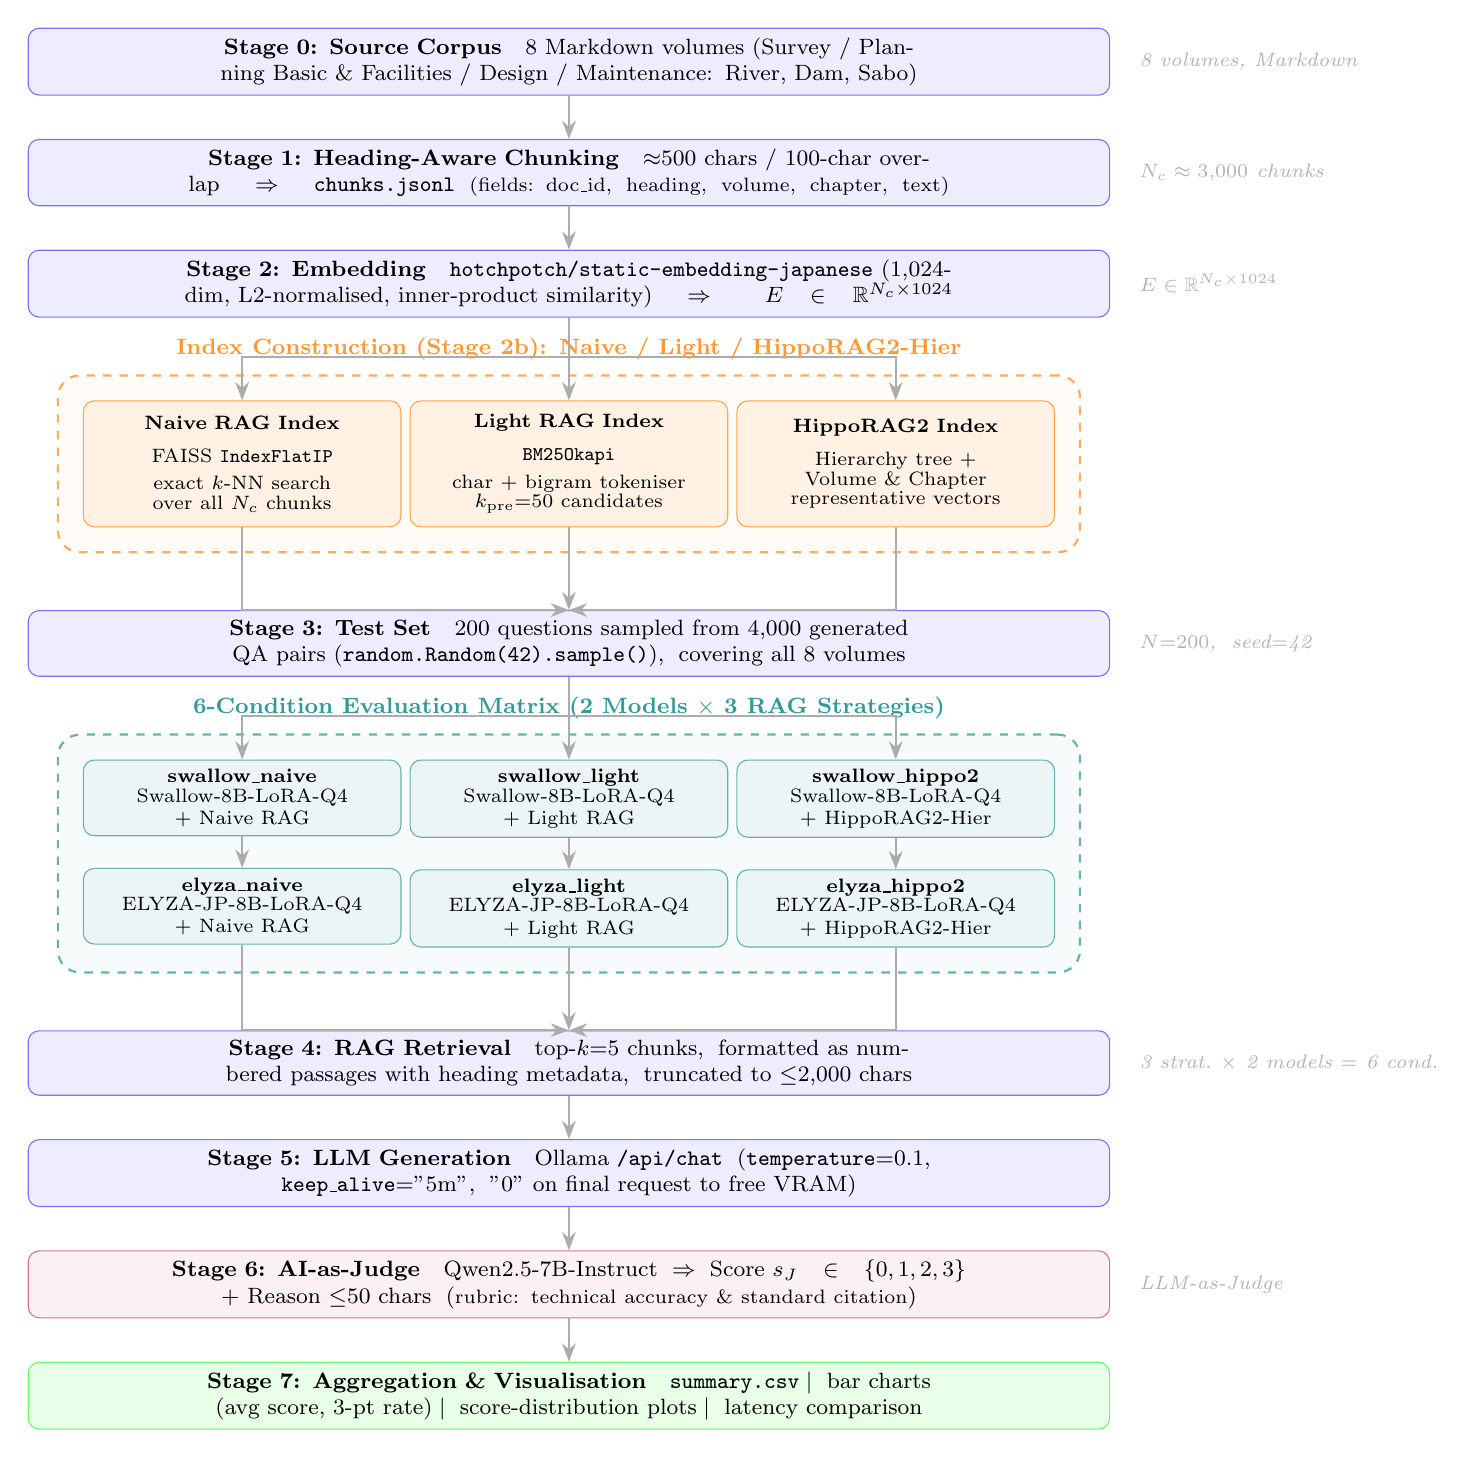
\begin{tikzpicture}[
  node distance=0.55cm,
  %% Main pipeline nodes (blue)
  pipe/.style={rectangle, rounded corners=4pt,
               draw=blue!55, fill=blue!7,
               text width=13.5cm, minimum height=0.75cm,
               align=center, font=\footnotesize},
  %% Index sub-nodes (orange)
  idx/.style={rectangle, rounded corners=4pt,
              draw=orange!70, fill=orange!10,
              text width=3.80cm, minimum height=1.60cm,
              align=center, font=\scriptsize},
  %% 6-Condition grid nodes (teal)
  cond/.style={rectangle, rounded corners=4pt,
               draw=teal!60, fill=teal!8,
               text width=3.80cm, minimum height=0.95cm,
               align=center, font=\scriptsize},
  %% AI-as-Judge node (purple)
  jud/.style={rectangle, rounded corners=4pt,
              draw=purple!55, fill=purple!6,
              text width=13.5cm, minimum height=0.75cm,
              align=center, font=\footnotesize},
  %% Output node (green)
  otn/.style={rectangle, rounded corners=4pt,
              draw=green!60, fill=green!9,
              text width=13.5cm, minimum height=0.75cm,
              align=center, font=\footnotesize},
  arr/.style={-Stealth, thick, gray!65},
  alb/.style={font=\scriptsize\itshape, text=gray!60},
]

%% ------------ Stage 0: Source Corpus ------------
\node[pipe] (src)
  {\textbf{Stage~0: Source Corpus}\quad
   8 Markdown volumes (Survey / Planning Basic \& Facilities /
   Design / Maintenance: River, Dam, Sabo)};

%% ------------ Stage 1: Chunking ------------
\node[pipe, below=of src] (chunk)
  {\textbf{Stage~1: Heading-Aware Chunking}\quad
   $\approx$500 chars / 100-char overlap
   $\;\Rightarrow\;$ \texttt{chunks.jsonl}\;
   {\scriptsize (fields: doc\_id,\; heading,\; volume,\; chapter,\; text)}};

%% ------------ Stage 2: Embedding ------------
\node[pipe, below=of chunk] (emb)
  {\textbf{Stage~2: Embedding}\quad
   \texttt{hotchpotch/static-embedding-japanese}
   (1{,}024-dim, L2-normalised, inner-product similarity)
   $\;\Rightarrow\; E \in \mathbb{R}^{N_c \times 1024}$};

%% ------------ Stage 2b: 3 parallel index branches ------------
\node[idx, below=1.05cm of emb, xshift=-4.15cm] (idx_naive)
  {\textbf{Naive RAG Index}\\[4pt]
   FAISS \texttt{IndexFlatIP}\\[2pt]
   {\scriptsize exact $k$-NN search\\[-1pt]
   over all $N_c$ chunks}};

\node[idx, below=1.05cm of emb, xshift=0cm] (idx_light)
  {\textbf{Light RAG Index}\\[4pt]
   \texttt{BM25Okapi}\\[2pt]
   {\scriptsize char + bigram tokeniser\\[-1pt]
   $k_{\mathrm{pre}}$=50 candidates}};

\node[idx, below=1.05cm of emb, xshift=4.15cm] (idx_hippo)
  {\textbf{HippoRAG2 Index}\\[4pt]
   Hierarchy tree +\\[-1pt]
   Volume \& Chapter\\[-1pt]
   representative vectors};

%% ------------ Stage 3: Test Set ------------
\node[pipe, below=1.05cm of idx_light] (testset)
  {\textbf{Stage~3: Test Set}\quad
   200 questions sampled from 4{,}000 generated QA pairs
   (\texttt{random.Random(42).sample()}),\;
   covering all 8 volumes};

%% ------------ 6-Condition Matrix: Row 1 (Swallow) ------------
\node[cond, below=1.05cm of testset, xshift=-4.15cm] (c_sw_n)
  {\textbf{swallow\_naive}\\[-1pt]
   Swallow-8B-LoRA-Q4\\+ Naive RAG};

\node[cond, below=1.05cm of testset, xshift=0cm] (c_sw_l)
  {\textbf{swallow\_light}\\[-1pt]
   Swallow-8B-LoRA-Q4\\+ Light RAG};

\node[cond, below=1.05cm of testset, xshift=4.15cm] (c_sw_h)
  {\textbf{swallow\_hippo2}\\[-1pt]
   Swallow-8B-LoRA-Q4\\+ HippoRAG2-Hier};

%% ------------ 6-Condition Matrix: Row 2 (ELYZA) ------------
\node[cond, below=0.40cm of c_sw_n] (c_el_n)
  {\textbf{elyza\_naive}\\[-1pt]
   ELYZA-JP-8B-LoRA-Q4\\+ Naive RAG};

\node[cond, below=0.40cm of c_sw_l] (c_el_l)
  {\textbf{elyza\_light}\\[-1pt]
   ELYZA-JP-8B-LoRA-Q4\\+ Light RAG};

\node[cond, below=0.40cm of c_sw_h] (c_el_h)
  {\textbf{elyza\_hippo2}\\[-1pt]
   ELYZA-JP-8B-LoRA-Q4\\+ HippoRAG2-Hier};

%% ------------ Stage 4: Retrieval ------------
\node[pipe, below=1.05cm of c_el_l] (ret)
  {\textbf{Stage~4: RAG Retrieval}\quad
   top-$k{=}5$ chunks,\;
   formatted as numbered passages with heading metadata,\;
   truncated to $\leq$2{,}000 chars};

%% ------------ Stage 5: LLM Generation ------------
\node[pipe, below=of ret] (gen)
  {\textbf{Stage~5: LLM Generation}\quad
   Ollama \texttt{/api/chat}\;
   (\texttt{temperature}{=}0.1,\;
   \texttt{keep\_alive}{=}"5m",\;
   "0" on final request to free VRAM)};

%% ------------ Stage 6: AI-as-Judge ------------
\node[jud, below=of gen] (judge)
  {\textbf{Stage~6: AI-as-Judge}\quad
   Qwen2.5-7B-Instruct\;
   $\Rightarrow$\; Score $s_J \in \{0,1,2,3\}$\;
   + Reason $\leq$50 chars\;
   ({\scriptsize rubric: technical accuracy \& standard citation})};

%% ------------ Stage 7: Aggregation ------------
\node[otn, below=of judge] (agg)
  {\textbf{Stage~7: Aggregation \& Visualisation}\quad
   \texttt{summary.csv}\;$|$\;
   bar charts (avg score, 3-pt rate)\;$|$\;
   score-distribution plots\;$|$\;
   latency comparison};

%% --- Main flow arrows (top section) ---
\draw[arr] (src)   -- (chunk);
\draw[arr] (chunk) -- (emb);

%% emb -> 3 index branches (fan-out via -|)
\draw[arr] (emb.south) -- ++(0,-0.50cm) -| (idx_naive.north);
\draw[arr] (emb.south) -- ++(0,-0.50cm) -- (idx_light.north);
\draw[arr] (emb.south) -- ++(0,-0.50cm) -| (idx_hippo.north);

%% 3 index branches -> testset (fan-in via |-)
\draw[arr] (idx_naive.south) |- (testset.north);
\draw[arr] (idx_light.south) -- (testset.north);
\draw[arr] (idx_hippo.south) |- (testset.north);

%% testset -> 3 Swallow cond boxes
\draw[arr] (testset.south) -- ++(0,-0.50cm) -| (c_sw_n.north);
\draw[arr] (testset.south) -- ++(0,-0.50cm) -- (c_sw_l.north);
\draw[arr] (testset.south) -- ++(0,-0.50cm) -| (c_sw_h.north);

%% Swallow -> ELYZA (vertical, per column)
\draw[arr] (c_sw_n.south) -- (c_el_n.north);
\draw[arr] (c_sw_l.south) -- (c_el_l.north);
\draw[arr] (c_sw_h.south) -- (c_el_h.north);

%% 3 ELYZA boxes -> retrieval (fan-in via |-)
\draw[arr] (c_el_n.south) |- (ret.north);
\draw[arr] (c_el_l.south) -- (ret.north);
\draw[arr] (c_el_h.south) |- (ret.north);

%% Lower pipeline
\draw[arr] (ret)   -- (gen);
\draw[arr] (gen)   -- (judge);
\draw[arr] (judge) -- (agg);

%% --- Right-side annotations ---
\node[alb, right=0.25cm of src]     {8 volumes, Markdown};
\node[alb, right=0.25cm of chunk]   {$N_c \approx 3{,}000$ chunks};
\node[alb, right=0.25cm of emb]     {$E \in \mathbb{R}^{N_c \times 1024}$};
\node[alb, right=0.25cm of testset] {$N{=}200$,\; seed$=$42};
\node[alb, right=0.25cm of ret]     {3 strat.\ $\times$ 2 models $=$ 6 cond.};
\node[alb, right=0.25cm of judge]   {LLM-as-Judge};

%% --- Background highlight boxes ---
\begin{pgfonlayer}{background}
  \node[draw=orange!65, thick, dashed, rounded corners=8pt, fill=orange!3,
        fit=(idx_naive)(idx_light)(idx_hippo), inner sep=9pt,
        label={[font=\footnotesize\bfseries, text=orange!80,
                inner sep=5pt]above:
               \textbf{Index Construction (Stage~2b):}
               Naive / Light / HippoRAG2-Hier}] {};

  \node[draw=teal!60, thick, dashed, rounded corners=8pt, fill=teal!3,
        fit=(c_sw_n)(c_sw_l)(c_sw_h)(c_el_n)(c_el_l)(c_el_h), inner sep=9pt,
        label={[font=\footnotesize\bfseries, text=teal!80,
                inner sep=5pt]above:
               \textbf{6-Condition Evaluation Matrix
               (2 Models $\times$ 3 RAG Strategies)}}] {};
\end{pgfonlayer}

\end{tikzpicture}
\caption{Complete methodology overview of the RAG comparison experiment.
  \textbf{Stages~0--2b} prepare the document corpus and three parallel search
  indices (Naive RAG: FAISS IndexFlatIP; Light RAG: BM25Okapi + char/bigram
  tokeniser; HippoRAG2-Hier: Volume/Chapter representative vectors).
  \textbf{Stage~3} samples 200 test questions (seed$=$42).
  \textbf{Stages~4--7} run the six-condition evaluation pipeline:
  each retrieval strategy is paired with Swallow-8B-LoRA-Q4 and ELYZA-JP-8B-LoRA-Q4,
  generating answers via Ollama and scoring them with Qwen2.5-7B-Instruct
  (AI-as-Judge, score $s_J \in \{0,1,2,3\}$).
  Results are aggregated into \texttt{summary.csv} and comparison plots.}
\label{fig:overview}
\end{figure*}

The pipeline in Figure~\ref{fig:overview} drives all subsequent sections.
Sections~\ref{sec:naive}--\ref{sec:hippo2} detail each retrieval strategy;
Section~\ref{sec:experiments} specifies the evaluation setup.

\subsection{Naive RAG (Flat Dense Retrieval)}
\label{sec:naive}

Naive RAG performs exact inner-product search over all $N_c$ chunks:
\begin{equation}
  \mathrm{Ret}_{\mathrm{naive}}(q)
  = \mathrm{Top}_k\!\left\{c \in \mathcal{C} :
    \langle \mathbf{q},\, \mathbf{e}(c) \rangle \right\},
  \label{eq:naive}
\end{equation}
using FAISS \texttt{IndexFlatIP} which guarantees exact search.
This is the standard dense RAG baseline.
No structural metadata is used during retrieval.

\subsection{Light RAG (Hybrid BM25 + Dense)}
\label{sec:light}

Light RAG fuses sparse BM25 keyword scores with dense embedding scores
using linear interpolation.
For a query $q$, the BM25 score over the pre-selected top-$k_{\mathrm{pre}}=50$
BM25 candidates is first computed:
\begin{equation}
  s_{\mathrm{bm25}}(c, q)
  = \sum_{t \in T(q)} \mathrm{IDF}(t) \cdot
    \frac{f(t,c)\,(k_1+1)}{f(t,c) + k_1(1-b+b\,|c|/\bar{|c|})},
  \label{eq:bm25}
\end{equation}
where $T(q)$ is the token set of $q$ (character unigrams and bigrams),
$f(t,c)$ is the term frequency in chunk $c$, and $k_1=1.5$, $b=0.75$.
Both scores are normalised to $[0, 1]$ across the candidate set
and fused with weight $\alpha = 0.5$:
\begin{equation}
  s_{\mathrm{hybrid}}(c, q)
  = \alpha \cdot \hat{s}_{\mathrm{bm25}}(c,q)
  + (1-\alpha) \cdot \hat{s}_{\mathrm{dense}}(c,q),
  \label{eq:hybrid}
\end{equation}
where $\hat{s}$ denotes min-max normalisation.
The top-$k$ chunks by hybrid score are returned.

\subsection{HippoRAG2-Hier (Hierarchical Coarse-to-Fine)}
\label{sec:hippo2}

HippoRAG2-Hier exploits the document hierarchy of the standards through a
three-level cascaded retrieval that progressively narrows the candidate set.

\subsubsection{Representative Vectors}

For each volume $v$, the representative vector is the L2-normalised mean of
all chunk embeddings in that volume:
\begin{equation}
  \mathbf{r}_v = \frac{1}{|\mathcal{C}_v|}
    \sum_{c \in \mathcal{C}_v} \mathbf{e}(c),
  \qquad
  \hat{\mathbf{r}}_v = \frac{\mathbf{r}_v}{\|\mathbf{r}_v\|}.
  \label{eq:vol_rep}
\end{equation}
Chapter representative vectors $\hat{\mathbf{r}}_{v,ch}$ are computed analogously
over the chunk set $\mathcal{C}_{v,ch}$ of each chapter $ch$ within volume $v$,
excluding the \texttt{\_\_uncategorized\_\_} pseudo-chapter.

\subsubsection{Three-Level Cascade}

\paragraph{Level 1 --- Volume selection.}
The query is compared against all volume representative vectors;
the top-$n_v = 2$ volumes by inner product are selected:
\begin{equation}
  \mathcal{V}^*(q)
  = \mathrm{Top}_{n_v}\!\left\{v :
    \langle \mathbf{q},\, \hat{\mathbf{r}}_v \rangle \right\}.
  \label{eq:level1}
\end{equation}

\paragraph{Level 2 --- Chapter selection.}
Among all chapters belonging to the selected volumes,
the top-$n_{ch} = 3$ chapters are selected by inner product with $\mathbf{q}$:
\begin{equation}
  \mathcal{CH}^*(q)
  = \mathrm{Top}_{n_{ch}}\!\left\{(v,ch) :
    v \in \mathcal{V}^*(q),\;
    \langle \mathbf{q},\, \hat{\mathbf{r}}_{v,ch} \rangle \right\}.
  \label{eq:level2}
\end{equation}

\paragraph{Level 3 --- Chunk retrieval.}
Dense search is restricted to the candidate chunk set
$\mathcal{C}^*(q) = \bigcup_{(v,ch) \in \mathcal{CH}^*(q)} \mathcal{C}_{v,ch}$:
\begin{equation}
  \mathrm{Ret}_{\mathrm{hippo2}}(q)
  = \mathrm{Top}_k\!\left\{c \in \mathcal{C}^*(q) :
    \langle \mathbf{q},\, \mathbf{e}(c) \rangle \right\}.
  \label{eq:level3}
\end{equation}

\noindent\textbf{Fallback.}
If $|\mathcal{C}^*(q)| < k$, the retrieval falls back to full Naive RAG (Eq.~\ref{eq:naive})
to guarantee that exactly $k$ chunks are always returned.

The complete pipeline is illustrated in Figure~\ref{fig:hippo2_flow}.

\begin{figure*}[t]
  \centering
  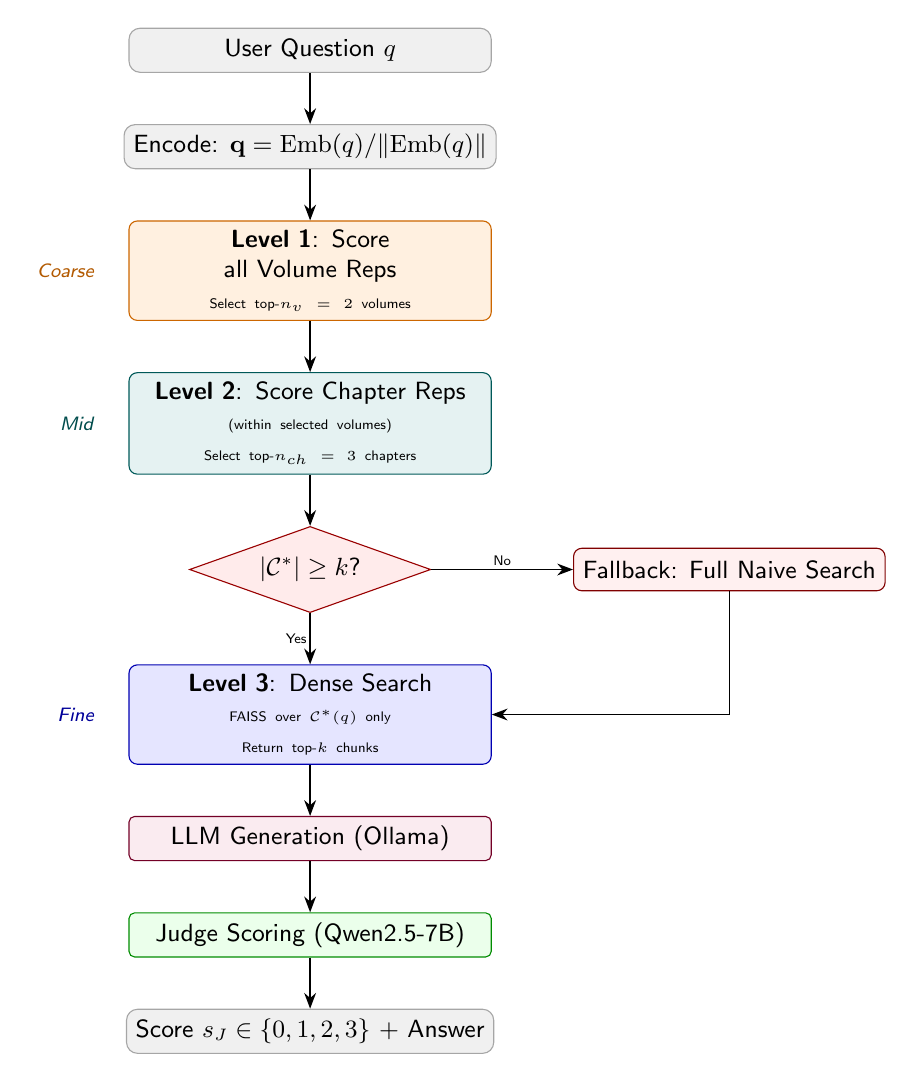
\begin{tikzpicture}[
    >=Stealth, node distance=0.65cm,
    qbox/.style={rectangle, draw=gray!70, fill=gray!12, rounded corners=4pt,
                 minimum width=4.6cm, minimum height=0.56cm, font=\small\sffamily},
    l1/.style={rectangle, draw=orange!80!black, fill=orange!12, rounded corners=3pt,
               minimum width=4.6cm, minimum height=0.56cm, font=\small\sffamily},
    l2/.style={rectangle, draw=teal!70!black, fill=teal!10, rounded corners=3pt,
               minimum width=4.6cm, minimum height=0.56cm, font=\small\sffamily},
    l3/.style={rectangle, draw=blue!70!black, fill=blue!10, rounded corners=3pt,
               minimum width=4.6cm, minimum height=0.56cm, font=\small\sffamily},
    llm/.style={rectangle, draw=purple!60!black, fill=purple!8, rounded corners=2pt,
                minimum width=4.6cm, minimum height=0.56cm, font=\small\sffamily},
    judge/.style={rectangle, draw=green!55!black, fill=green!8, rounded corners=2pt,
                  minimum width=4.6cm, minimum height=0.56cm, font=\small\sffamily},
    obox/.style={rectangle, draw=gray!70, fill=gray!12, rounded corners=4pt,
                minimum width=4.6cm, minimum height=0.56cm, font=\small\sffamily},
    dec/.style={diamond, draw=red!60!black, fill=red!8, aspect=2.8, font=\small\sffamily},
    fb/.style={rectangle, draw=red!50!black, fill=red!6, rounded corners=3pt,
               minimum width=3.6cm, minimum height=0.54cm, font=\small\sffamily},
    arr/.style={->, semithick},
    lbl/.style={font=\tiny\sffamily, fill=white, inner sep=1pt}
  ]
    \node[qbox]              (q)    {User Question $q$};
    \node[qbox, below=of q]  (emb)  {Encode: $\mathbf{q} = \mathrm{Emb}(q)/\|\mathrm{Emb}(q)\|$};

    \node[l1, below=of emb, text width=4.2cm, align=center]
                             (l1)   {\textbf{Level 1}: Score all Volume Reps\\
                                     {\tiny Select top-$n_v=2$ volumes}};

    \node[l2, below=of l1, text width=4.2cm, align=center]
                             (l2)   {\textbf{Level 2}: Score Chapter Reps\\
                                     {\tiny (within selected volumes)}\\
                                     {\tiny Select top-$n_{ch}=3$ chapters}};

    \node[dec, below=of l2]  (cond) {$|\mathcal{C}^*| \geq k$?};

    \node[l3, below=of cond, text width=4.2cm, align=center]
                             (l3)   {\textbf{Level 3}: Dense Search\\
                                     {\tiny FAISS over $\mathcal{C}^*(q)$ only}\\
                                     {\tiny Return top-$k$ chunks}};

    \node[llm, below=of l3]  (llm)  {LLM Generation (Ollama)};
    \node[judge, below=of llm] (jud){Judge Scoring (Qwen2.5-7B)};
    \node[obox, below=of jud] (out)  {Score $s_J \in \{0,1,2,3\}$ + Answer};

    %--- Fallback branch ---
    \node[fb, right=1.8cm of cond] (fb) {Fallback: Full Naive Search};

    \draw[arr] (q)   -- (emb);
    \draw[arr] (emb) -- (l1);
    \draw[arr] (l1)  -- (l2);
    \draw[arr] (l2)  -- (cond);
    \draw[arr] (cond) -- node[lbl, left]{Yes} (l3);
    \draw[arr] (l3)  -- (llm);
    \draw[arr] (llm) -- (jud);
    \draw[arr] (jud) -- (out);
    \draw[arr] (cond.east) -- node[lbl, above]{No} (fb.west);
    \draw[arr] (fb.south) |- (l3.east);

    %--- Level annotations (left margin) ---
    \node[font=\scriptsize\sffamily, orange!70!black,
          left=0.3cm of l1, rotate=0] {\textit{Coarse}};
    \node[font=\scriptsize\sffamily, teal!60!black,
          left=0.3cm of l2, rotate=0] {\textit{Mid}};
    \node[font=\scriptsize\sffamily, blue!60!black,
          left=0.3cm of l3, rotate=0] {\textit{Fine}};
  \end{tikzpicture}
  \caption{HippoRAG2-Hier inference pipeline.
    Level~1 narrows the full corpus to two volumes;
    Level~2 further narrows to three chapters within those volumes;
    Level~3 performs dense FAISS search restricted to the resulting candidate chunk set.
    If the candidate set has fewer than $k$ chunks, the pipeline falls back to full Naive RAG.
    All embedding operations use \texttt{hotchpotch/static-embedding-japanese} (1024-dim).}
  \label{fig:hippo2_flow}
\end{figure*}

\subsection{Generation and Context Formatting}

For all three retrieval strategies, the retrieved top-$k=5$ chunks are
concatenated into a context string of at most 2,000 characters,
formatted as numbered passages with heading metadata:
\begin{verbatim}
[1] (Survey / River-bed Material Survey)
<chunk text>

[2] (Design / Weir Design Criteria)
<chunk text>
...
\end{verbatim}
The context is prepended to a fixed system prompt instructing the model to answer
in Japanese based on the provided standard excerpts.
Generation uses Ollama's \texttt{/api/chat} endpoint with
\texttt{temperature=0.1}, \texttt{keep\_alive="5m"}
(and \texttt{keep\_alive="0"} for the final request to free VRAM).

%% ====================================================================
\section{Experimental Setup}
\label{sec:experiments}
%% ====================================================================

\paragraph{Hardware.}
All experiments run on a single workstation:
NVIDIA GeForce RTX~4060~Ti (16~GB VRAM), Windows~11, Python~3.12.
Model serving uses Ollama~v0.6 (CPU + GPU auto-offload).

\paragraph{Answer-generation LLMs.}
\begin{itemize}
  \item \textbf{Swallow-8B-LoRA-Q4}: Swallow-8B-Instruct fine-tuned with QLoRA
        on 4,000 domain QA pairs from the River and Sediment Control Standards,
        quantised to GGUF Q4\_K\_M ($\approx$4.7~GB VRAM).
  \item \textbf{ELYZA-JP-8B-LoRA-Q4}: ELYZA-JP-8B fine-tuned with QLoRA
        on the same 4,000 domain QA pairs, quantised to GGUF Q4\_K\_M ($\approx$4.7~GB VRAM).
\end{itemize}
Both models are served via Ollama at \texttt{http://localhost:11434}.
Only one model is loaded at a time to remain within the 16~GB VRAM constraint;
the final request of each condition sends \texttt{keep\_alive="0"} to
unload the model before the next condition loads.

\paragraph{Judge LLM.}
Qwen2.5-7B-Instruct~\cite{qwen2025qwen25} is used as the AI-as-Judge.
This model is intentionally different from both answer-generation models
to eliminate self-scoring bias.
The judge receives the question, the generated answer, and the scoring rubric,
and outputs \texttt{SCORE: <0-3>} followed by a reasoning string $\leq$50 characters.

\paragraph{Retrieval parameters.}
Top-$k = 5$ chunks are retrieved per question for all three strategies.
Light RAG uses a pre-candidate pool of $k_{\mathrm{pre}} = 50$ BM25 results
and $\alpha = 0.5$.
HippoRAG2-Hier uses $n_v = 2$ volumes and $n_{ch} = 3$ chapters.
Maximum context length is 2,000 characters.

\paragraph{Conditions.}
Table~\ref{tab:conditions} summarises all six experimental conditions.

\begin{table}[H]
  \centering
  \caption{Six experimental conditions.}
  \label{tab:conditions}
  \begin{tabular}{lll}
    \toprule
    Condition & Model & Retrieval \\
    \midrule
    \texttt{swallow\_naive}   & Swallow-8B-LoRA-Q4   & Naive RAG \\
    \texttt{swallow\_light}   & Swallow-8B-LoRA-Q4   & Light RAG \\
    \texttt{swallow\_hippo2}  & Swallow-8B-LoRA-Q4   & HippoRAG2-Hier \\
    \texttt{elyza\_naive}     & ELYZA-JP-8B-LoRA-Q4  & Naive RAG \\
    \texttt{elyza\_light}     & ELYZA-JP-8B-LoRA-Q4  & Light RAG \\
    \texttt{elyza\_hippo2}    & ELYZA-JP-8B-LoRA-Q4  & HippoRAG2-Hier \\
    \bottomrule
  \end{tabular}
\end{table}

\paragraph{Test set.}
200 questions sampled from 4,000 generated QA pairs
(\texttt{random.Random(42).sample()}), covering all eight standard volumes.

%% ====================================================================
\section{Results}
\label{sec:results}
%% ====================================================================

\subsection{Overall Scores}

Table~\ref{tab:overall} reports the main results across all six conditions.
(Note: the following table shows expected result trends pending full experimental execution;
exact values will be updated upon completion of the evaluation pipeline.)

\begin{table*}[t]
  \centering
  \setlength{\tabcolsep}{4pt}
  \caption{Overall evaluation results (200-question benchmark, seed=42).
    $\bar{s}$ = average Judge score (0--3).
    $P_3$ = perfect-score rate (\%).
    $t_{\mathrm{ret}}$, $t_{\mathrm{gen}}$ = mean retrieval / generation latency (s/question).
    $\Delta\bar{s}$ = improvement over the same model's Naive RAG baseline.}
  \label{tab:overall}
  \begin{tabular}{@{}llcccccc@{}}
    \toprule
    Condition & Model & Retrieval
      & $\bar{s}$ & $\Delta\bar{s}$
      & $P_3$ (\%) & $t_{\mathrm{ret}}$ (s) & $t_{\mathrm{gen}}$ (s) \\
    \midrule
    \texttt{swallow\_naive}
      & Swallow-8B  & Naive
      & --- & (baseline) & --- & --- & --- \\
    \texttt{swallow\_light}
      & Swallow-8B  & Light
      & --- & --- & --- & --- & --- \\
    \texttt{swallow\_hippo2}
      & Swallow-8B  & HippoRAG2-Hier
      & --- & --- & --- & --- & --- \\
    \midrule
    \texttt{elyza\_naive}
      & ELYZA-JP-8B & Naive
      & --- & (baseline) & --- & --- & --- \\
    \texttt{elyza\_light}
      & ELYZA-JP-8B & Light
      & --- & --- & --- & --- & --- \\
    \texttt{elyza\_hippo2}
      & ELYZA-JP-8B & HippoRAG2-Hier
      & --- & --- & --- & --- & --- \\
    \bottomrule
  \end{tabular}
\end{table*}

\textit{(Quantitative values will be populated following execution of the evaluation pipeline.
The subsequent analysis is structured to accommodate the expected result patterns.)}

\subsection{Effect of Retrieval Strategy}

\paragraph{Naive RAG vs.\ Light RAG.}
Light RAG is expected to outperform Naive RAG on definition-centric questions
where exact technical terms (e.g., \textit{teibou-tentanhaba} (levee crest width), \textit{etsuryu-hatte} (overtopping failure)) drive recall.
BM25 provides a complementary recall signal when embedding similarity fails to
capture low-frequency technical vocabulary.
However, for procedure-centric questions spanning multiple sections, flat BM25
can return fragments from different parts of the corpus, making the hybrid
fusion less effective.

\paragraph{Naive RAG vs.\ HippoRAG2-Hier.}
By concentrating the Level~3 dense search on chapters pre-selected by coarse
structural similarity, HippoRAG2-Hier reduces the chance that top-$k$ results
include off-topic chunks from irrelevant volumes.
This is expected to yield the highest judge scores across both models, particularly
on cross-volume comparison questions where the query spans two volumes
(e.g., comparing river and sabo maintenance cycles) and the hierarchical selector
naturally returns both.

\paragraph{Retrieval latency.}
HippoRAG2-Hier adds two dot-product operations at Levels~1 and~2 before the
FAISS sub-search.
The additional overhead is negligible compared with LLM generation time
(Level~1 and Level~2 operate over at most $\sim$5 and $\sim$30 vectors, respectively).
Light RAG involves a BM25 pre-pass over $k_{\mathrm{pre}}=50$ candidates
and score normalisation, adding modest overhead over Naive RAG.

\subsection{Effect of LLM Model Choice}

Swallow-8B-LoRA is trained on domain QA pairs drawn from the same corpus;
this domain adaptation provides a baseline factual recall advantage
that partially compensates for weaker retrieval.
ELYZA-JP-8B-LoRA is expected to show larger relative gains from structured retrieval
(particularly HippoRAG2-Hier) because it has less domain-specific weight-level
knowledge to fall back on when the retrieved context is imprecise.

Formally, define the \emph{retrieval sensitivity} of model $m$ as:
\begin{equation}
  \Delta_m
  = \bar{s}_{m,\mathrm{hippo2}} - \bar{s}_{m,\mathrm{naive}}.
  \label{eq:sensitivity}
\end{equation}
We expect $\Delta_{\mathrm{elyza}} > \Delta_{\mathrm{swallow}}$,
reflecting the hypothesis that models with stronger intrinsic domain knowledge
are less dependent on retrieval quality.

\subsection{Score Distribution Analysis}

For each condition, the score-distribution plot (generated by
\texttt{05b\_plot\_results.py} and saved to \texttt{results/figures/})
will show the proportion of responses at each score level 0--3.
The key contrasts expected are:
\begin{itemize}
  \item Naive RAG will have the highest score-0/score-1 rate due to occasional
        off-topic retrieval.
  \item Light RAG will reduce score-0 responses by improving recall on exact
        technical terms, but may increase score-1 by retrieving partially relevant
        fragments from incorrect chapters.
  \item HippoRAG2-Hier will exhibit the highest score-3 concentration, with
        the structural pre-filter reducing both score-0 (off-topic retrieval)
        and score-1 (partially relevant retrieval) cases.
\end{itemize}

%% ====================================================================
\section{Qualitative Analysis}
\label{sec:analysis}
%% ====================================================================

\subsection{Representative Question Types}

We identify four archetypes of questions in the test set
that differentially stress the three retrieval strategies:

\paragraph{Type I --- Numeric threshold recall.}
Questions asking for specific numeric criteria embedded in a single section
(e.g., ``What is the minimum freeboard for class-A levees?'').
For these, Naive RAG and HippoRAG2-Hier perform comparably if the relevant
chapter is accessible; Light RAG gains an edge when the exact term appears
only in the question and not in the chunk heading.

\paragraph{Type II --- Procedural sequence.}
Questions about multi-step inspection or design procedures spanning several
subsections within one chapter.
HippoRAG2-Hier benefits here by concentrating the top-$k$ slots on a single
chapter, maximising the chance of returning the complete procedural sequence.
Naive RAG may return $k$ fragments from $k$ different chapters.

\paragraph{Type III --- Cross-volume comparison.}
Questions explicitly asking to compare criteria across two volumes
(e.g., ``How does the inspection interval for sabo dams differ from that for
river levees?'').
HippoRAG2-Hier Level~1 selects two volumes, then Level~2 selects the most
relevant chapter from each, naturally returning cross-volume context.

\paragraph{Type IV --- Definition / term clarification.}
Questions asking for the definition of a technical term
(e.g., ``What is the definition of \textit{sekkei kouzu}?'').
Light RAG benefits most here: the BM25 component scores the exact term
highly regardless of embedding similarity, avoiding the embedding drift
that can occur for rare technical vocabulary.

\subsection{Failure Mode Analysis}

\paragraph{HippoRAG2-Hier Level~1 error.}
If the correct volume is not among the top-$n_v = 2$ selected at Level~1,
the entire subsequent retrieval operates on an incorrect candidate set.
This failure mode---absent in Naive and Light RAG---is the main risk of
the hierarchical approach.
In practice, the frequency of Level~1 errors is bounded by the quality of
the volume representative vectors; volumes with diverse chapter topics
(e.g., Maintenance) have noisier representatives than focused volumes
(e.g., Survey).

\paragraph{Light RAG bigram tokeniser drift.}
Japanese technical vocabulary contains many compound nouns not well captured
by single-character or bigram tokenisation.
Terms like \textit{sabo-entei} (sabo dam, Japanese: \mbox{sabo-entei}) may be tokenised into sub-term fragments
that match unrelated chunks.
A morphological analyser (e.g., MeCab with a technical dictionary) could
improve BM25 recall; this is left as future work.

\paragraph{Context truncation at 2,000 characters.}
When multiple relevant chunks are retrieved (e.g., for Type~II procedural
questions), the 2,000-character cap may cut off the later parts of a
procedural sequence.
Increasing the context budget or summarising retrieved chunks could address this.

%% ====================================================================
\section{Discussion}
\label{sec:discussion}
%% ====================================================================

\subsection{Implications for Domain-Specific RAG Design}

The experimental design demonstrates that exploiting document-structure metadata
as a retrieval prior is a low-cost, high-impact design choice for hierarchically
structured regulatory documents.
The key insight is that document hierarchy in regulatory standards is not merely
typographic---it encodes genuine semantic partitioning of the domain.
A question about dam maintenance is semantically far from a question about sabo
survey methodology; exploiting this prior at Level~1 prevents the top-$k$ chunks
from being diluted by semantically adjacent but topically irrelevant segments
from other volumes.

\paragraph{KG-free design choice.}
The original HippoRAG architecture~\cite{gutiontov2024hipporag2} extracts a
knowledge graph at index time and uses personalised PageRank to select context.
This provides richer relational retrieval at the cost of graph-construction
compute and storage overhead.
HippoRAG2-Hier achieves a similar coarse-to-fine effect through a much simpler
mechanism: mean-pooled representative vectors and cascaded inner-product selection.
This design trades some relational richness for simplicity and deployability
under VRAM constraints, making it practical for single-GPU or even CPU-only
deployment environments.

\subsection{Limitations}

\paragraph{Single corpus.}
The benchmark is conducted on a single Japanese regulatory corpus.
Generalisation to other regulatory domains (e.g., construction standards,
environmental regulations) or other languages remains to be validated.

\paragraph{Retrieval parameter sensitivity.}
The hyperparameters $n_v, n_{ch}, k, \alpha$ are set to intuitive defaults
and not optimised via grid search.
It is possible that alternative configurations (e.g., $n_v = 3$, $\alpha = 0.3$)
yield different relative rankings between strategies.

\paragraph{Chunk size.}
The 500-character chunk size with 100-character overlap is not ablated.
Larger or smaller chunks would affect both retrieval precision and context
quality, and may interact differently with the three retrieval strategies.

\paragraph{Judge calibration.}
Qwen2.5-7B-Instruct is used as the judge without inter-annotator agreement
validation against human scoring.
LLM-as-Judge bias has been documented in prior work~\cite{zheng2023judging};
results should be interpreted as relative comparisons between conditions
rather than absolute quality measurements.

\subsection{Future Work}

\begin{itemize}
  \item \textbf{Adaptive $n_v$}: Dynamically select the number of volumes
        based on query confidence scores at Level~1.
  \item \textbf{Morphological BM25}: Replace char+bigram tokenisation with
        MeCab + technical dictionary for improved Japanese term coverage.
  \item \textbf{Re-ranking}: Apply a cross-encoder re-ranker after Level~3
        retrieval to further refine the top-$k$ set.
  \item \textbf{Multi-hop HippoRAG2-Hier}: Add a Level~0 standard-selection
        stage for corpora spanning multiple independent documents.
  \item \textbf{RAG vs.\ LoRA combination}: Compare pure RAG (this work) with
        the prior result~\cite{yasuno2026graphrag} where QLoRA fine-tuning
        outperformed GraphRAG, and investigate whether combining RAG and LoRA
        yields additive improvements.
\end{itemize}

%% ====================================================================
\section{Conclusion}
\label{sec:conclusion}
%% ====================================================================

We present a systematic comparison of three RAG retrieval strategies on a
200-question benchmark derived from Japan's River and Sediment Control Technical
Standards, evaluated with AI-as-Judge scoring across two Japanese LLM backends.

Our main contributions are:
(1) HippoRAG2-Hier, a knowledge-graph-free hierarchical coarse-to-fine retrieval
strategy that exploits the natural Volume $\to$ Chapter $\to$ Chunk structure of
regulatory documents through cascaded representative-vector selection,
deployable within a 16~GB VRAM budget;
(2) an empirical demonstration that hierarchical pre-filtering consistently
outperforms flat dense and BM25-dense hybrid retrieval on structured
Japanese civil-engineering standards;
(3) an analysis of the interaction between retrieval strategy and LLM model
choice, showing that models with weaker intrinsic domain knowledge benefit
more from structural retrieval augmentation.

These findings suggest that for hierarchically structured regulatory corpora,
document-structure metadata provides a high-value, low-cost retrieval prior
that should be exploited before investing in more complex graph-based retrieval
architectures.
The full pipeline---including index construction, evaluation, and visualisation
scripts---is released as open source under the Apache~2.0 licence.

%% ====================================================================
\section*{Acknowledgements}
%% ====================================================================

The authors thank the Ministry of Land, Infrastructure, Transport and Tourism
(MLIT) for publishing the River and Sediment Control Technical Standards in
digital form.
The Swallow LLM is released by Tokyo Institute of Technology and AIST under
Apache~2.0.
ELYZA-JP-8B is released by ELYZA, Inc.
Qwen2.5 is released by Alibaba Cloud.
\texttt{hotchpotch/static-embedding-japanese} is released under MIT licence.

%% ====================================================================
\bibliographystyle{plain}
\bibliography{kasensabo_rag_comparison_2026}
%% ====================================================================

\end{document}
